%%%%%%%%%%% Aquí va la solución al problema 1.
\newpage\textbf{\textcolor{MidnightBlue}{2.}}
Demuestra que el algoritmo 2 soluciona el problema del consenso en una gráfica G arbitraria, tolerando
$f < k(G)$ fallas de tipo paro. $k(G)$ denota la conexidad por vértices de G, es decir, el mínimo
número de vértices que se tienen que quitar de $G$ para desconectarla. Entonces, si hay menos de $k(G)$
fallas de los procesos, la gráfica que queda sigue siendo conexa. Tip: Piensa que tanto tarda en fluir la
entrada mínima más pequeña, a pesar de las fallas que puedan ocurrir.\\


\begin{center}
    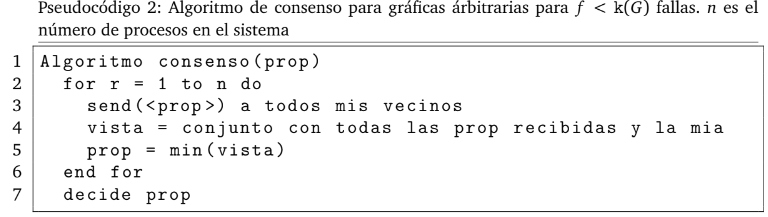
\includegraphics[scale=0.6]{consensoProblema2.png}
\end{center}

$\rhd$ Para mostrar que el algoritmo 2 soluciona el consenso, mostremos que
%\newcommand{\localtextbulletone}{\textcolor{black}{\raisebox{.45ex}{\rule{.6ex}{.6ex}}}}
%\renewcommand{\labelitemi}{\localtextbulletone}
\begin{itemize}
\item \textit{Terminación.} Si $f < k(G)$ entonces $G$ siempre será conexa incluso si
      los $f$ procesos fallan. Por tanto, los procesos que hayan logrado el consenso
      hasta antes del último fallo en los $f$ procesos enviarán nuevamente su conjunto
      con $ID's$ y su propuesta de consenso, como la gráfica sigue siendo conexa,
      eventualmente todos los procesos tendrán la vista de todos los demás que no tuvieron
      fallas de tipo paro y la propuesta de cada proceso será tomada en cuenta para
      el consenso de los $G - f$ procesos restantes.
\item \textit{Validez.} El consenso se originó en alguno de los procesos, por tanto
      es válido.
\item \textit{Acuerdo.} En cuanto termine el algoritmo todos los procesos activos están
      conectados y tienen la misma propuesta de consenso. De no ser así, falta un proceso
      por enviar su consenso y el \code{for} no ha llegado a su fin, esto contradice el hecho
      de que nuestro algoritmo haya terminado, por tanto se cumple que todos los procesos
      llegan al acuerdo en cuanto se termine el algoritmo (pues la función \code{min} es
      determinista).
\end{itemize}
\hfill $\lhd$
\newline
